\subsection{整体架构}
\label{sec:core:arch}

\begin{figure}[htbp]
\centering
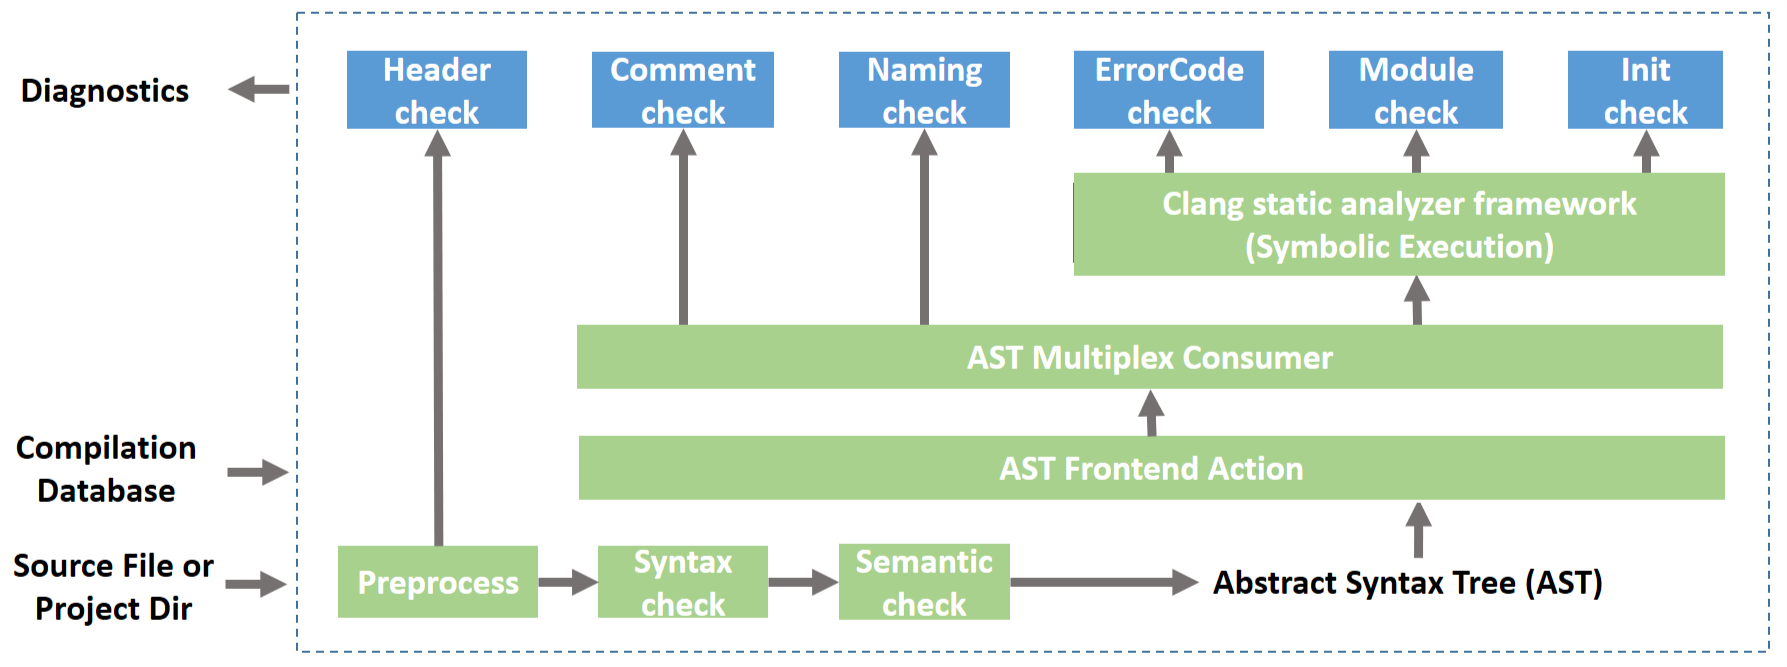
\includegraphics[width=\textwidth]{figure/architecture}
\caption{工具整体架构图}
\label{fig:arch}
\end{figure}

本工具整体基于\href{https://clang.llvm.org/}{Clang}框架扩展实现。
\autoref{fig:arch}展示了本工具的软件架构,
它接收待检查的源文件或项目目录与编译源文件使用的{\bf 编译命令数据库}(可选)作为输入,
检测和识别源文件中存在的违反编码规范的潜在缺陷,最后输出相应的诊断信息。
当输入为项目目录时,工具会递归地收集目录下所有的源文件依次处理。
\autoref{fig:arch}中以矩形色块表示对数据的操作,
绿色底色的矩形属于Clang框架提供的编译分析基础设施,
蓝色底色的矩形属于根据竞赛六点需求在Clang提供的基础设施上研制的相应检查。

输入工具的C程序文件会依次经历预处理、
语法检查和语义检查最终生成抽象语法树
(Abstract Syntax Tree, 简称AST)。
竞赛需求中有关头文件的相关检查(Header Check)
在预处理阶段通过\textbf{预处理器回调机制}实现;
其余五点需求通过AST结构上的一个前端动作(Frontend Action)的\textbf{多路AST消费者}来实现。
在五点需求中,
函数头注释检查(Comment Check)和命名检查(Naming Check)
直接实现为\href{https://clang.llvm.org/doxygen/classclang_1_1ASTConsumer.html}{ASTConsumer}子类,
而函数错误处理检查(ErrorCode Check)、模块内外调用规范检查(Module Check)
和按需初始化检查(Init Check)则
使用\href{https://clang-analyzer.llvm.org/}{Clang静态分析框架}进行\textbf{基于符号执行的路径敏感的过程内分析}。
针对输入的每个源文件和一条可能的编译命令,
工具只会对该源文件解析一次,六项检查会在这一次解析过程中依次完成。

后续六节会依次介绍各点需求实现策略,
\S\ref{sec:core:header}介绍需求一“头文件应当自包含,且没有循环依赖”的实现;
\S\ref{sec:core:arg}介绍需求二“模块内部函数参数的合法性检查,由调用者负责”的实现;
\S\ref{sec:core:error}介绍需求三“对函数的错误返回码要全面处理”的实现;
\S\ref{sec:core:naming}介绍需求四“除了常见的、通用缩写外,不使用单词缩写,不得使用汉语拼音”的实现;
\S\ref{sec:core:comment}介绍需求五“函数命名无法表达的信息,必须加函数头注释辅助说明”的实现;
\S\ref{sec:core:init}介绍需求六“变量或内存块,按需初始化;禁止冗余清零”的实现。
